\documentclass[11pt,a4paper]{article}
\usepackage[T1]{fontenc}
\usepackage[utf8]{inputenc}
\usepackage{lmodern}
\usepackage{textcomp}
\usepackage[left=1.8cm,right=1.8cm,top=3.0cm,bottom=2.2cm,headheight=36pt,headsep=12pt]{geometry}
\usepackage{multicol}
\usepackage{xcolor}
\usepackage{fancyhdr}\usepackage{tikz}
\usepackage{graphicx}
\usepackage{array}
\usepackage{amsmath,amssymb}
\usepackage{setspace}
\usepackage{longtable}
\graphicspath{{../}}
\definecolor{ygreen}{RGB}{46,139,87}\definecolor{dgreen}{RGB}{28,90,56}
\renewcommand{\normalsize}{\fontsize{10.9}{13.4}\selectfont}
\renewcommand{\familydefault}{\rmdefault}
\setlength{\parindent}{0pt}
\setlength{\columnsep}{0.8cm}
\setlength{\columnseprule}{0.4pt}
\setlength{\multicolsep}{3pt plus 1pt minus 1pt}
\renewcommand{\textsubscript}[1]{\ensuremath{_{\text{\fontsize{8}{8}\selectfont #1}}}}
\renewcommand{\textsuperscript}[1]{\ensuremath{^{\text{\fontsize{8}{8}\selectfont #1}}}}
\newcommand{\qn}[1]{\textbf{\fontsize{11.5}{13}\selectfont #1}}
\newcommand{\qsep}{\par\vspace{13pt}}
\newcommand{\fwrule}{\par\vspace{5pt}\noindent\rule{\linewidth}{1.4pt}\par\vspace{7pt}}
\newsavebox{\fitb}
\newcommand{\fitbox}[1]{\sbox{\fitb}{#1}\ifdim\wd\fitb>\linewidth\resizebox{\linewidth}{!}{\usebox{\fitb}}\else\usebox{\fitb}\fi}
\newcommand{\diqqat}[1]{\par\smallskip\noindent\textbf{Diqqat!} #1\par\medskip}
\newcommand{\javob}{\par\nopagebreak[4]\smallskip\noindent\textbf{Javob:} \rule[-2pt]{7.5cm}{0.4pt}\par\smallskip\noindent\textbf{Diqqat!} Javobingizni javoblar varaqasiga ko`chirib yozing.\par\medskip}
\pagestyle{fancy}
\fancyhf{}
\renewcommand{\headrulewidth}{1.6pt}\renewcommand{\headrule}{{\color{ygreen}\hrule height 1.6pt width\headwidth}}
\newcommand{\hdrlogo}{
\begin{tikzpicture}[baseline=0pt]\fill[ygreen,rounded corners=3pt] (0,0) rectangle (0.95,0.95);\node[white,font=\fontsize{24}{26}\bfseries\selectfont] at (0.475,0.47){K};\node[anchor=west,font=\fontsize{16}{18}\bfseries\selectfont,text=dgreen] at (1.15,0.66){KIMYO};\node[anchor=west,font=\footnotesize\scshape,text=gray] at (1.15,0.2){Milliy sertifikat\ \ 2026};\end{tikzpicture}}
\newcommand{\hdrpill}[1]{\begin{tikzpicture}[baseline=0pt]\node[fill=ygreen,text=white,rounded corners=8pt,inner xsep=10pt,inner ysep=5pt,font=\fontsize{13}{15}\bfseries\selectfont] at (0,0.475){#1};\end{tikzpicture}}
\fancyhead[L]{\hdrlogo}
\fancyhead[R]{\hdrpill{18-variant}}

\fancyfoot[C]{\thepage}
\fancypagestyle{first}{\fancyhf{}\renewcommand{\headrulewidth}{1.6pt}\renewcommand{\headrule}{{\color{ygreen}\hrule height 1.6pt width\headwidth}}\fancyhead[L]{\hdrlogo}\fancyhead[R]{\hdrpill{18-variant}}\fancyfoot[C]{\thepage}}
\begin{document}
\normalsize
\thispagestyle{first}
\noindent\textit{Davriy jadvaldan foydalanish mumkin.}
\par\smallskip
\begin{multicols}{2}
\noindent\qn{1.} 7,3 g HCl 200 g suvda eritildi. Eritmaning molyal \textbf{konsentratsiyasini (mol/kg) aniqlang.}

\noindent A)~\textsl{0,96} \hfill B)~\textsl{1} \hfill C)~\textsl{0} \hfill D)~\textsl{2}\par
\qsep
\noindent\qn{2.} 1 M H\textsubscript{2}SO\textsubscript{4} eritmasining normal \textbf{konsentratsiyasini (n) aniqlang.}

\noindent A)~\textsl{1} \hfill B)~\textsl{4} \hfill C)~\textsl{0,5} \hfill D)~\textsl{2}\par
\qsep
\noindent\qn{3.} H\textsubscript{2}O\textsubscript{2} tarkibida O ning oksidlanish \textbf{darajasini aniqlang.}

\noindent A)~\textsl{+2} \hfill B)~\textsl{+3 va +5} \hfill C)~\textsl{+7} \hfill D)~\textsl{$-$1}\par
\qsep
\noindent\qn{4.} HCHO molekulasidagi $\sigma$ va $\pi$ bog`lar \textbf{sonini aniqlang.}

\noindent A)~\textsl{2 va 1} \hfill B)~\textsl{3 va 1} \hfill C)~\textsl{3 va 2} \hfill D)~\textsl{4 va 1}\par
\qsep
\noindent\qn{5.} Rasmda molekulaning sharsimon modeli tasvirlangan (yashil -- C, sariq -- H, qizil -- O, ko`k -- N).
\begin{center}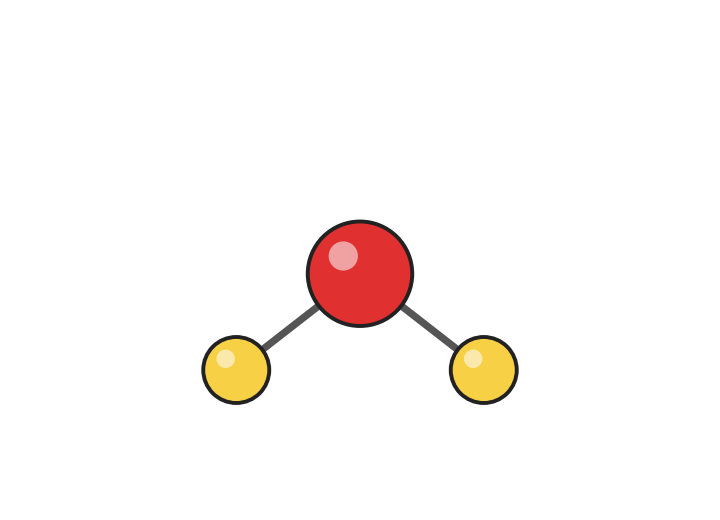
\includegraphics[width=0.86\linewidth]{rasmlar/gen/md_2012.png}\end{center}
Molekula fazoviy shakli qanday?

\noindent\begin{tabular}{@{}p{0.47\linewidth}@{}p{0.47\linewidth}@{}}
A)~\textsl{uchburchakli piramida} & B)~\textsl{chiziqli} \\
C)~\textsl{burchakli} & D)~\textsl{tetraedr} \\
\end{tabular}\par
\qsep
\noindent\qn{6.} Na\textsubscript{2}SO\textsubscript{4} ning suvli eritmasi inert elektrodlar bilan elektroliz qilinganda qaysi moddalar ajraladi?

\noindent\begin{tabular}{@{}p{0.47\linewidth}@{}p{0.47\linewidth}@{}}
A)~\textsl{H\textsubscript{2} va O\textsubscript{2}} & B)~\textsl{H\textsubscript{2}, Cl\textsubscript{2} va NaOH} \\
C)~\textsl{Cu va O\textsubscript{2}} & D)~\textsl{Cu va Cl\textsubscript{2}} \\
\end{tabular}\par
\qsep
\noindent\qn{7.} Faqat oksidlovchi bo`la oladigan \textbf{ionlarni aniqlang}: 1) I\textsuperscript{$-$}; 2) Fe\textsuperscript{3+}; 3) Zn\textsuperscript{2+}; 4) Cl\textsuperscript{$-$}

\noindent A)~\textsl{1, 3} \hfill B)~\textsl{4} \hfill C)~\textsl{2} \hfill D)~\textsl{3}\par
\qsep
\noindent\qn{8.} Radioaktiv izotopning boshlang`ich miqdorining 7/8 qismi parchalandi. Necha yarim yemirilish davri o`tgan?

\noindent A)~\textsl{4} \hfill B)~\textsl{2} \hfill C)~\textsl{6} \hfill D)~\textsl{3}\par
\qsep
\noindent\qn{9.} H\textsubscript{2} + I\textsubscript{2} $\rightleftarrows$ 2HI sistemasida boshlang`ich moddalarning har biridan 4 mol dan 5 l hajmli idishga solindi. Muvozanat qaror topganda reagentlarning har birining 1/2 qismi sarflangan bo`ldi. Muvozanat \textbf{konstantasini hisoblang.}

\noindent A)~\textsl{8} \hfill B)~\textsl{2} \hfill C)~\textsl{5} \hfill D)~\textsl{4}\par
\qsep
\noindent\qn{10.} Na\textsubscript{2}SO\textsubscript{4} eritmasiga 0,2 mol/l li BaCl\textsubscript{2} eritmasi oz-ozdan qo`shilganda hosil bo`lgan cho`kma massasining qo`shilgan hajmga bog`liqligi grafikda keltirilgan.
\begin{center}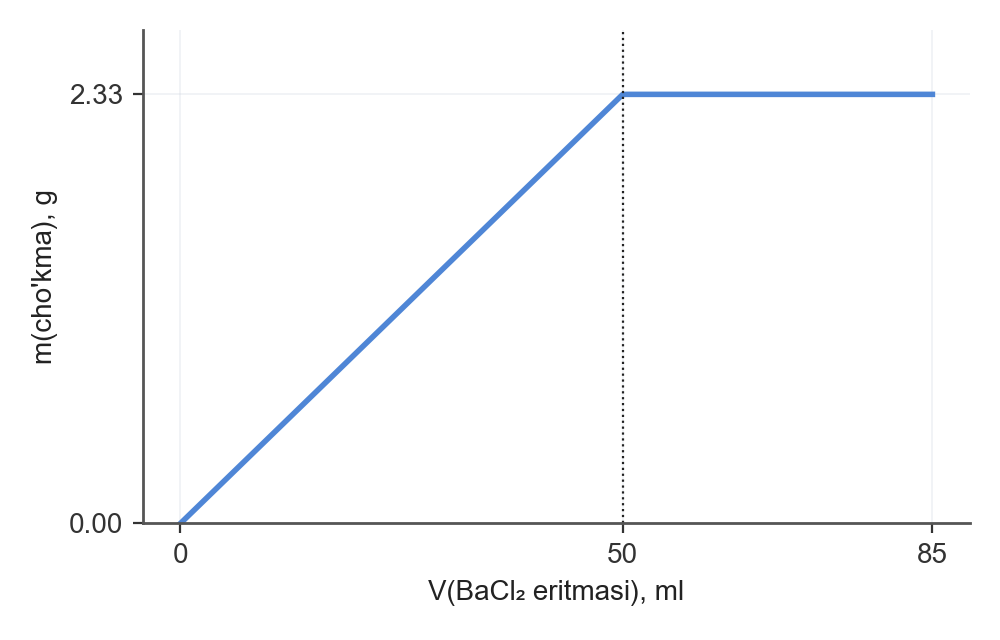
\includegraphics[width=0.86\linewidth]{rasmlar/gen/pp_v18_0.png}\end{center}
Grafikdagi cho`kma massasi 2,33 g da to`xtagan. Egri chiziq to`xtagan nuqtagacha qo`shilgan BaCl\textsubscript{2} ning \textbf{massasini (g) toping.}

\noindent A)~\textsl{2,33} \hfill B)~\textsl{1,42} \hfill C)~\textsl{2,08} \hfill D)~\textsl{4,16}\par
\qsep
\noindent\qn{11.} 2NO + O\textsubscript{2} $\rightleftarrows$ 2NO\textsubscript{2} reaksiyasi 2 l hajmli idishda o`tkazildi. Ma'lumotlar jadvalda berilgan:
\begin{center}
\renewcommand{\arraystretch}{1.15}
\fitbox{\begin{tabular}{|c|c|c|c|}\hline
\textbf{Modda} & \textbf{NO} & \textbf{O\textsubscript{2}} & \textbf{NO\textsubscript{2}} \\ \hline
Boshlang`ich, mol & 6 & 6 & 0 \\ \hline
Muvozanatda, mol & --- & --- & 4 \\ \hline
\end{tabular}}
\end{center}
Muvozanat \textbf{konstantasini (K) hisoblang.}

\noindent A)~\textsl{4} \hfill B)~\textsl{1} \hfill C)~\textsl{2} \hfill D)~\textsl{0,5}\par
\qsep
\noindent\qn{12.} Quyidagi jadvalda NaNO\textsubscript{3} tuzining eritmalari keltirilgan:
\begin{center}
\renewcommand{\arraystretch}{1.15}
\fitbox{\begin{tabular}{|c|c|c|}\hline
\textbf{No.} & \textbf{m(eritma), g} & \textbf{$\omega$, \%} \\ \hline
I & 50 & 12 \\ \hline
II & 300 & 30 \\ \hline
\end{tabular}}
\end{center}
Eritmalar aralashtirilib, ustiga 50 g suv qo`shildi. Oxirgi eritmadagi tuzning massa \textbf{ulushini (\%) toping.}

\noindent A)~\textsl{21} \hfill B)~\textsl{42} \hfill C)~\textsl{14,57} \hfill D)~\textsl{24}\par
\qsep
\noindent\qn{13.} 23,8 g massali 238-massa sonli izotop (\textit{Z} = 92) 8 ta $\alpha$- va 6 ta $\beta$\textsuperscript{$-$}-yemirilishga uchradi (M $\approx$ 238 g/mol). Chiqarilgan $\alpha$-zarralar sonini N\textsubscript{A} birligida \textbf{aniqlang.}

\noindent A)~\textsl{0,8} \hfill B)~\textsl{0,6} \hfill C)~\textsl{1,4} \hfill D)~\textsl{0,1}\par
\qsep
\noindent\qn{14.} Probirkalardagi eritmalar: NaCl, Na\textsubscript{2}SO\textsubscript{4}, Na\textsubscript{2}CO\textsubscript{3} ni alohida probirkalarda ajratish uchun qaysi reagent(lar) yetarli? 1) lakmus; 2) HCl va lakmus; 3) HCl va BaCl\textsubscript{2}; 4) BaCl\textsubscript{2}

\noindent A)~\textsl{2, 3} \hfill B)~\textsl{3} \hfill C)~\textsl{1, 2} \hfill D)~\textsl{4}\par
\qsep
\noindent\qn{15.} Ishqoriy metallar haqida qaysi fikrlar to`g`ri? 1) KOH -- kuchli ishqor; 2) Natriy yonganda Na\textsubscript{2}O\textsubscript{2} hosil bo`ladi; 3) Natriy suv bilan reaksiyada H\textsubscript{2} va NaOH hosil qiladi; 4) Natriyning olinishi suyuqlanma NaCl elektrolizi bilan

\noindent\begin{tabular}{@{}p{0.47\linewidth}@{}p{0.47\linewidth}@{}}
A)~\textsl{1, 2, 3, 4} & B)~\textsl{1, 2, 4} \\
C)~\textsl{2, 3, 4} & D)~\textsl{1, 3, 4} \\
\end{tabular}\par
\qsep
\noindent\qn{16.} 6 mol H\textsubscript{2}S 6 mol kislorodda yondirildi (H\textsubscript{2}S to`liq sarflandi; oltingugurt va SO\textsubscript{2} aralashmasi hosil bo`ldi). Hosil bo`lgan oltingugurtning \textbf{massasini (g) hisoblang.}

\noindent A)~\textsl{192} \hfill B)~\textsl{96} \hfill C)~\textsl{48} \hfill D)~\textsl{144}\par
\qsep
\noindent\qn{17.} Si va SiO\textsubscript{2} dan iborat 14,8 g aralashma mo`l NaOH eritmasi bilan qizdirilganda 4,48 l (n.sh.) vodorod ajraldi. Reagent (NaOH) eritmasining massa ulushi 20\% va zichligi 1,4 g/ml; u mo`l miqdorda olingan. Aralashmani to`liq eritish uchun sarflangan NaOH \textbf{massasini (g) hisoblang.}

\noindent A)~\textsl{24} \hfill B)~\textsl{8} \hfill C)~\textsl{16} \hfill D)~\textsl{12}\par
\qsep
\noindent\qn{18.} Ca va CaC\textsubscript{2} dan iborat aralashma suv bilan ta'sirlashganda 6,72 l (n.sh.) gaz aralashmasi ajraldi, uning vodorodga nisbatan zichligi 9. Dastlabki aralashmaning \textbf{massasini (g) hisoblang.}

\noindent A)~\textsl{16,8} \hfill B)~\textsl{33,6} \hfill C)~\textsl{8,4} \hfill D)~\textsl{10,4}\par
\qsep
\noindent\qn{19.} NH\textsubscript{3} + HCl $\to$ NH\textsubscript{4}Cl reaksiyasida 8,96 l (n.sh.) NH\textsubscript{3} ishtirok etdi (unum 50\%). Barcha reaksiyalar 1 atm bosimda olib borildi. NH\textsubscript{4}Cl \textbf{massasini (g) toping.}

\noindent A)~\textsl{21,4} \hfill B)~\textsl{5,35} \hfill C)~\textsl{16,05} \hfill D)~\textsl{10,7}\par
\qsep
\noindent\qn{20.} Aldegid va ketonlar haqida qaysi fikrlar to`g`ri? 1) Aldegidlar "kumush ko`zgu" reaksiyasini beradi; 2) Formaldegid gaz holatda, suvda yaxshi eriydi; 3) Aseton Cu(OH)\textsubscript{2} ni qaytaradi; 4) Sirka aldegid Kucherov reaksiyasi bilan olinadi

\noindent A)~\textsl{1, 3, 4} \hfill B)~\textsl{1, 2, 4} \hfill C)~\textsl{1, 2, 3} \hfill D)~\textsl{2, 3, 4}\par
\qsep
\noindent\qn{21.} Karbon kislotalar haqida qaysi fikrlar to`g`ri? 1) Sirka kislota karbonatlar bilan CO\textsubscript{2} ajratadi; 2) Benzoy kislota Na\textsubscript{2}CO\textsubscript{3} bilan reaksiyaga kirishmaydi; 3) Karboksil guruh karbonil va gidroksil guruhlardan iborat; 4) Olein kislota Br\textsubscript{2} ni biriktiradi

\noindent A)~\textsl{2, 4} \hfill B)~\textsl{2, 3} \hfill C)~\textsl{3, 4} \hfill D)~\textsl{1, 3, 4}\par
\qsep
\noindent\qn{22.} Aminlar, aminokislotalar va oqsillar haqida qaysi fikrlar to`g`ri? 1) Glitsin optik faol; 2) Aminlar kuchsiz asoslar xossasini namoyon qiladi; 3) Dipeptidda 2 ta peptid bog` bor; 4) Anilin bromli suv bilan oq cho`kma beradi

\noindent A)~\textsl{2, 4} \hfill B)~\textsl{1, 4} \hfill C)~\textsl{3, 4} \hfill D)~\textsl{1}\par
\qsep
\noindent\qn{23.} Metilformiat va etilatsetat aralashmasi (41,6 g) mo`l NaOH eritmasi bilan to`liq gidrolizlandi. Aralashmaning mol miqdori 0,6 mol. Aralashmadagi etilatsetat \textbf{massasini (g) toping.}

\noindent A)~\textsl{24} \hfill B)~\textsl{35,2} \hfill C)~\textsl{17,6} \hfill D)~\textsl{20,8}\par
\qsep
\noindent\qn{24.} 810 g kraxmal gidrolizlanib (unum 75\%) glukoza olindi, glukoza esa spirtli bijg`ishga uchradi (unum 80\%). Hosil bo`lgan etanol \textbf{massasini (g) toping.}

\noindent A)~\textsl{276} \hfill B)~\textsl{138} \hfill C)~\textsl{552} \hfill D)~\textsl{345}\par
\qsep
\noindent\qn{25.} 224 l (n.sh.) C\textsubscript{3}H\textsubscript{8} dan quyidagi sxema bo`yicha 74,24 g aseton olindi: C\textsubscript{3}H\textsubscript{8} $\to$ CH\textsubscript{3}--CH=CH\textsubscript{2} $\to$ CH\textsubscript{3}--CH(OH)--CH\textsubscript{3} $\to$ CH\textsubscript{3}--CO--CH\textsubscript{3}. Dastlabki 2 bosqichning unumi ketma-ket 80\%, 40\% ga teng. Barcha reaksiyalar 1,5 atm bosimda olib borildi. Oxirgi bosqichning \textbf{unumini (\%) aniqlang.}

\noindent A)~\textsl{20} \hfill B)~\textsl{40} \hfill C)~\textsl{60} \hfill D)~\textsl{32}\par
\qsep
\noindent\qn{26.} CaC\textsubscript{2} dan quyidagi sxema bo`yicha 14,34 g polivinilxlorid olindi: CaC\textsubscript{2} $\to$ C\textsubscript{2}H\textsubscript{2} $\to$ CH\textsubscript{2}=CHCl $\to$ (--CH\textsubscript{2}--CHCl--)n. Bosqichlarning unumi ketma-ket 85\%, 90\%, 75\% ni tashkil qiladi. Texnik CaC\textsubscript{2} tarkibida 80\% sof modda bor. Barcha reaksiyalar 1 atm bosimda olib borildi. Sarflangan texnik CaC\textsubscript{2} massasi (g) \textbf{ni aniqlang.}

\noindent A)~\textsl{64} \hfill B)~\textsl{16} \hfill C)~\textsl{32} \hfill D)~\textsl{27,2}\par
\qsep
\noindent\qn{27.} Texnik CaC\textsubscript{2} tarkibida 75\% sof modda bor. 128 g CaC\textsubscript{2} dan quyidagi sxema bo`yicha etanol olindi: CaC\textsubscript{2} $\to$ C\textsubscript{2}H\textsubscript{2} $\to$ C\textsubscript{2}H\textsubscript{4} $\to$ C\textsubscript{2}H\textsubscript{5}OH. Bosqichlarning unumi ketma-ket 75\%, 85\%, 80\% ni tashkil qiladi. Barcha reaksiyalar 1,5 atm bosimda olib borildi. Olingan etanol \textbf{massasini (g) aniqlang.}

\noindent A)~\textsl{70,38} \hfill B)~\textsl{17,59} \hfill C)~\textsl{35,19} \hfill D)~\textsl{43,99}\par
\qsep
\noindent\qn{28.} C\textsubscript{4}H\textsubscript{9}OH va C\textsubscript{3}H\textsubscript{7}OH aralashmasi tarkibida aralashmadagi protonlarning umumiy soni 16$\cdot$N\textsubscript{A}. Aralashmaning massasi 28,2 g. Aralashmadagi C\textsubscript{4}H\textsubscript{9}OH ning mol \textbf{ulushini (\%) hisoblang.}

\noindent A)~\textsl{25} \hfill B)~\textsl{78,72} \hfill C)~\textsl{75} \hfill D)~\textsl{50}\par
\qsep
\noindent\qn{29.} 684 g C\textsubscript{12}H\textsubscript{22}O\textsubscript{11} dan quyidagi sxema bo`yicha 250,24 g etanol olindi: C\textsubscript{12}H\textsubscript{22}O\textsubscript{11} $\to$ C\textsubscript{6}H\textsubscript{12}O\textsubscript{6} (glyukoza va fruktoza) $\to$ C\textsubscript{2}H\textsubscript{5}OH. Dastlabki 1 bosqichning unumi ketma-ket 80\% ga teng. Barcha reaksiyalar 1,5 atm bosimda olib borildi. Oxirgi bosqichning \textbf{unumini (\%) aniqlang.}

\noindent A)~\textsl{42} \hfill B)~\textsl{85} \hfill C)~\textsl{15} \hfill D)~\textsl{68}\par
\qsep
\noindent\qn{30.} 200 g 10\% li va 100 g 40\% li NaOH eritmalari aralashtirildi. Yangi eritmaning massa \textbf{ulushini (\%) toping.}

\noindent A)~\textsl{25} \hfill B)~\textsl{50} \hfill C)~\textsl{20} \hfill D)~\textsl{18}\par
\qsep
\noindent\qn{31.} Rasmdagi tajribada fenolftalein qo`shilgan suvga ammiak yuttirildi, eritma pushti rangga kirdi. Bu nimani ko`rsatadi?
\begin{center}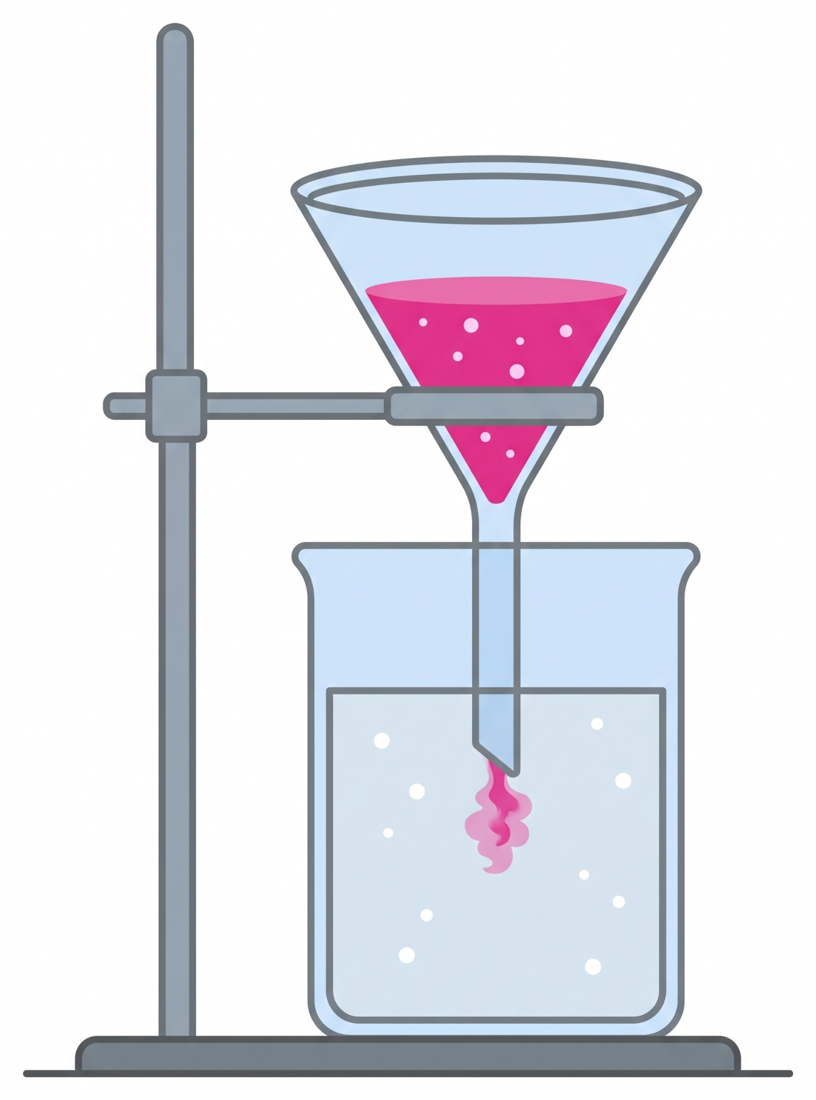
\includegraphics[width=0.86\linewidth]{rasmlar/darslik/d_nh3_fontan.png}\end{center}
\noindent A)~\textsl{NH\textsubscript{3} havodan og`ir}\par
\noindent B)~\textsl{NH\textsubscript{3} suvda yaxshi eriydi va eritma ishqoriy xossaga ega}\par
\noindent C)~\textsl{NH\textsubscript{3} suvda erimaydi, eritma kislotali}\par
\noindent D)~\textsl{NH\textsubscript{3} suvda erimaydi, eritma neytral}\par
\qsep
\noindent\qn{32.} Raqamlangan (1--4) probirkalarda AgNO\textsubscript{3}, HCl, Na\textsubscript{2}CO\textsubscript{3}, NaOH eritmalari tartibsiz holda berilgan. Quyidagi kuzatuvlar asosida moddalarni probirka raqami bilan moslang. 1- va 2-probirkalardagi eritmalar aralashtirilganda oq-sarg`ish cho`kma tushadi. 3- va 4-probirkalardagi eritmalar aralashtirilganda bir-birini neytrallaydi. 1- va 3-probirkalardagi eritmalar aralashtirilganda to`q qo`ng`ir cho`kma tushadi.
\noindent A)~\textsl{1-AgNO\textsubscript{3}, 2-Na\textsubscript{2}CO\textsubscript{3}, 3-NaOH, 4-HCl}\par
\noindent B)~\textsl{1-AgNO\textsubscript{3}, 2-HCl, 3-NaOH, 4-Na\textsubscript{2}CO\textsubscript{3}}\par
\noindent C)~\textsl{1-AgNO\textsubscript{3}, 2-NaOH, 3-Na\textsubscript{2}CO\textsubscript{3}, 4-HCl}\par
\noindent D)~\textsl{1-Na\textsubscript{2}CO\textsubscript{3}, 2-AgNO\textsubscript{3}, 3-NaOH, 4-HCl   ---}\par
\qsep
\end{multicols}
\medskip
\noindent\setlength{\fboxsep}{0pt}\fbox{\begin{tabular}{p{0.74\linewidth}|p{0.2\linewidth}}
\parbox[t]{0.72\linewidth}{\vspace{3pt}\textbf{Topshiriqlar (33--35) va javob variant (A--F)larini o`zaro to`g`ri moslashtiring.} Qo`rg`oshin(II) nitratning 0,01 mol/l li eritmasidan 500 ml olinib, inert elektrodlar yordamida 5 A tok kuchi bilan 96 s elektroliz qilindi (eritma hajmi o`zgarmadi deb hisoblang). Elektrolizdan keyin eritmaga mo`l KI eritmasi qo`shildi.
\vspace{3pt}} & \parbox[t]{0.19\linewidth}{\vspace{3pt}A~\textsl{2,3}\\[3pt]
B~\textsl{0,52}\\[3pt]
C~\textsl{2}\\[3pt]
D~\textsl{3,46}\\[3pt]
E~\textsl{3}\\[3pt]
F~\textsl{0,41}}\\ \hline
\parbox[t]{0.72\linewidth}{\vspace{2pt}\textbf{33. Katodda ajralgan qo`rg`oshin massasini (g) toping.}\vspace{2pt}} & \\ \hline
\parbox[t]{0.72\linewidth}{\vspace{2pt}\textbf{34. Elektroliz tugagach eritmaning pH ini hisoblang.}\vspace{2pt}} & \\ \hline
\parbox[t]{0.72\linewidth}{\vspace{2pt}\textbf{35. KI qo`shilganda hosil bo`lgan cho`kma massasini (g) aniqlang.}\vspace{2pt}} & 
\end{tabular}}
\par\bigskip
\noindent\qn{36.} 5\% li va 15\% li tuz eritmalari massalar nisbati 1 : 1 bo`lgan holda aralashtirildi. Tajriba laboratoriyada, kvars idishda o`tkazildi. Hosil bo`lgan eritmaning massa \textbf{ulushini (\%) hisoblang.}
\javob\qsep
\noindent\qn{37.} 300 g 8\% li tuz eritmasidan suv bug`latilganda tuzning massa ulushi 3/2 marta ortdi. Tajriba hajmi 500 ml bo`lgan kolbada o`tkazildi. Bug`latilgan suv \textbf{massasini (g) toping.}
\javob\qsep
\noindent\qn{38.} Cu va CuO dan iborat 7,2 g aralashma mo`l suyultirilgan H\textsubscript{2}SO\textsubscript{4} da ishlandi, 3,2 g qattiq qoldiq qoldi. Aralashmaning zichligi 2,3 g/sm\textsuperscript{3} ga teng. Hosil bo`lgan tuz \textbf{massasini (g) aniqlang.}
\javob\qsep
\noindent\qn{39.} Noma'lum alkenning 22,4 g miqdori mo`l brom suvi bilan to`liq reaksiyaga kirishganda 64 g brom sarflandi. Xuddi shu alkenning 3/4 qismi gidratlanib spirtga aylantirildi, hosil bo`lgan spirt natriy bilan ta'sirlashtirildi. Reagent (brom suvi) eritmasining massa ulushi 20\% va zichligi 1,4 g/ml; u mo`l miqdorda olingan. Ajralgan vodorod \textbf{hajmini (l, n.sh.) toping.}
\javob\qsep
\noindent\qn{40.} Vodorodga nisbatan zichligi 22 bo`lgan alkanning 88 g miqdorining 3/4 qismi yorug`likda xlor bilan monoxlorlandi, hosil bo`lgan xloralkan mo`l KOH ning suvli eritmasi bilan gidrolizlandi. Reagent (KOH) eritmasining massa ulushi 36\% va zichligi 1,05 g/ml; u mo`l miqdorda olingan. Hosil bo`lgan spirtning \textbf{massasini (g) toping.}
\javob\qsep
\par\bigskip\begin{center}\textbf{\fontsize{13}{15}\selectfont YOZMA ISH}\end{center}
\noindent\qn{41.} \textbf{Topshiriqni bajarish jarayonida barcha reaksiya tenglamalarini yozing. Miqdoriy va arifmetik hisoblashlarni (unga asos bo`lgan usul yoki formulani ko`rsatgan holda) uzviy ketma-ketlikda bajaring.}\par\smallskip
500 g suvda CuSO\textsubscript{4} va NaCl dan iborat 33,55 g aralashma eritildi (tuzlarning mol nisbati 1 : 3). Elektrolizyorning hajmi 2 l. Eritma inert elektrodlar yordamida 10 A tok kuchi bilan 4825 s elektroliz qilindi (jarayonda Cu\textsuperscript{2+} va Cl\textsuperscript{$-$} ionlari to`liq tugadi, suv ham elektrolizga uchradi).\par
\noindent 1)\ Katod va anodda ketma-ket boradigan jarayonlar tenglamalarini yozing; tuzlarning dastlabki miqdorlarini (mol) aniqlang.\par
\noindent 2)\ Katodda ajralgan mis massasini (g) va vodorod hajmini (l, n.sh.) hisoblang.\par
\noindent 3)\ Anodda ajralgan xlor va kislorod hajmlarini (l, n.sh.) toping.\par
\noindent 4)\ Elektroliz tugagach eritmaning muhitini (kislotali, neytral yoki ishqoriy) asoslang va undagi ortiqcha moddaning miqdorini (mol) aniqlang.\par
\noindent 5)\ Elektrolizdan keyin eritma massasini (g) va undagi Na\textsubscript{2}SO\textsubscript{4} ning massa ulushini (\%) hisoblang.\par
\diqqat{Mazkur topshiriq kengaytirilgan javobni talab etib, uning yechilish usuli va shu usul asosidagi barcha hisoblash amallari javoblar varaqasida aks etishi lozim.}\qsep
\noindent\qn{42.} Organik moddalarning xossalarini bilgan holda reaksiya tenglamalarini tugallang va tenglashtiring. 3- va 5-reaksiyalarda hosil bo`lgan asosiy organik mahsulotlarni sistematik nomenklatura bo`yicha nomlang. Hosil bo`lgan organik moddalarning tuzilish formulalarini yozing.\par
\noindent 1)\ CH\textsubscript{3}--CH\textsubscript{2}--OH + CH\textsubscript{3}--COOH (H\textsubscript{2}SO\textsubscript{4}, t) $\rightleftarrows$\par
\noindent 2)\ HCOOCH\textsubscript{3} + NaOH (t) $\to$\par
\noindent 3)\ C\textsubscript{6}H\textsubscript{5}--CH\textsubscript{3} + KMnO\textsubscript{4} + H\textsubscript{2}SO\textsubscript{4} (t) $\to$\par
\noindent 4)\ H\textsubscript{2}N--CH\textsubscript{2}--COOH + H\textsubscript{2}N--CH\textsubscript{2}--COOH $\to$\par
\noindent 5)\ H\textsubscript{2}N--CH\textsubscript{2}--COOH + HCl $\to$\par
\noindent 6)\ CH\textsubscript{3}--CHO + H\textsubscript{2} (Ni, t) $\to$\par
\noindent 7)\ CH\textsubscript{3}--CH=CH\textsubscript{2} + KMnO\textsubscript{4} + H\textsubscript{2}O (0 \textdegree{}C) $\to$\par
\diqqat{Mazkur topshiriq kengaytirilgan javobni talab etib, uning yechilish usuli va shu usul asosidagi barcha hisoblash amallari javoblar varaqasida aks etishi lozim.}\qsep
\noindent\qn{43.} \textbf{Topshiriqni bajarish jarayonida barcha reaksiya tenglamalarini yozing. Miqdoriy va arifmetik hisoblashlarni (unga asos bo`lgan usul yoki formulani ko`rsatgan holda) uzviy ketma-ketlikda bajaring.}\par\smallskip
Alyuminiy va noma'lum \textit{X} metalldan (\textit{X} -- oksidlanish darajasi +2 bo`lgan metall) iborat 7,8 g aralashma mo`l NaOH eritmasi bilan ta'sirlashganda 6,72 l (n.sh.) gaz ajraldi. Shunday massali ikkinchi namuna mo`l xlorid kislotada eritilganda 8,96 l (n.sh.) gaz ajraldi. Xlorid kislotali eritmaga mo`l NaOH eritmasi qo`shilib, cho`kma ajratildi, havoda to`liq oksidlanguncha tutildi va kuydirildi; filtratdan mo`l CO\textsubscript{2} o`tkazildi. Reagent (NaOH) eritmasining massa ulushi 50\% va zichligi 1,4 g/ml; u mo`l miqdorda olingan. Hosil bo`lgan Al(OH)\textsubscript{3} nitrat kislotada eritildi, eritma bug`latilib, qoldiq doimiy massagacha qizdirildi, ajralgan gazlar suvga yuttirildi.\par
\noindent 1)\ Barcha reaksiyalarning tenglamalarini yozing va tenglashtiring.\par
\noindent 2)\ Aralashmadagi Al va \textit{X} ning miqdorlarini (mol) aniqlang va \textit{X} metallni toping.\par
\noindent 3)\ Aralashmadagi metallarning massa ulushlarini (\%) hisoblang. Al(OH)\textsubscript{3} ni eritish uchun sarflangan HNO\textsubscript{3} miqdorini (mol) toping.\par
\noindent 4)\ Kuydirishdan hosil bo`lgan qattiq moddaning formulasini aniqlang va massasini (g) hisoblang. Al(NO\textsubscript{3})\textsubscript{3} qizdirilganda ajralgan gazlar hajmini (l, n.sh.) hisoblang.\par
\noindent 5)\ Filtratdan CO\textsubscript{2} o`tkazilganda hosil bo`lgan cho`kma massasini (g) toping. Gazlar suvga yuttirilganda hosil bo`lgan HNO\textsubscript{3} massasini (g) aniqlang.\par
\diqqat{Mazkur topshiriq kengaytirilgan javobni talab etib, uning yechilish usuli va shu usul asosidagi barcha hisoblash amallari javoblar varaqasida aks etishi lozim.}\qsep
\newpage
\noindent\textbf{\fontsize{13}{15}\selectfont 18-variant}\hfill \textbf{Javoblar kaliti}\par\smallskip\hrule\smallskip
\textit{Faqat o`qituvchi uchun.}\par\medskip
\noindent\textbf{1--32-savollar}\par\smallskip
\noindent\begin{tabular}{|c|c|c|c|c|c|c|c|c|c|c|c|c|c|c|c|}\hline
\textbf{1} & \textbf{2} & \textbf{3} & \textbf{4} & \textbf{5} & \textbf{6} & \textbf{7} & \textbf{8} & \textbf{9} & \textbf{10} & \textbf{11} & \textbf{12} & \textbf{13} & \textbf{14} & \textbf{15} & \textbf{16}\\\hline
\textsl{B} & \textsl{D} & \textsl{D} & \textsl{B} & \textsl{C} & \textsl{A} & \textsl{D} & \textsl{D} & \textsl{D} & \textsl{C} & \textsl{C} & \textsl{D} & \textsl{A} & \textsl{B} & \textsl{A} & \textsl{B}\\\hline
\textbf{17} & \textbf{18} & \textbf{19} & \textbf{20} & \textbf{21} & \textbf{22} & \textbf{23} & \textbf{24} & \textbf{25} & \textbf{26} & \textbf{27} & \textbf{28} & \textbf{29} & \textbf{30} & \textbf{31} & \textbf{32}\\\hline
\textsl{A} & \textsl{A} & \textsl{D} & \textsl{B} & \textsl{D} & \textsl{A} & \textsl{C} & \textsl{A} & \textsl{B} & \textsl{C} & \textsl{C} & \textsl{C} & \textsl{B} & \textsl{C} & \textsl{B} & \textsl{A}\\\hline
\end{tabular}\par\medskip
\noindent\textbf{33--35-savollar}\par\smallskip
\noindent\begin{tabular}{|c|c|c|}\hline \textbf{No} & \textbf{Javob} & \textbf{Qiymat}\\\hline
33 & \textsl{B} & 0,52\\\hline
34 & \textsl{C} & 2\\\hline
35 & \textsl{A} & 2,3\\\hline
\end{tabular}\par\medskip
\noindent\textbf{36--40-savollar}\par\smallskip
\noindent\begin{tabular}{|c|c|}\hline \textbf{No} & \textbf{To`g`ri javob}\\\hline
36 & 10\\\hline
37 & 100\\\hline
38 & 8\\\hline
39 & 3,36\\\hline
40 & 90\\\hline
\end{tabular}\par\medskip
\noindent\textbf{41--43-topshiriqlar: javoblar}\par\smallskip
\noindent\textbf{41-topshiriq.}\par
\noindent 1) 0,1 mol; 0,3 mol\par
\noindent 2) 6,4 g; 0,15 mol = 3,36 l\par
\noindent 3) 3,36 l; 1,12 l\par
\noindent 4) ishqoriy; NaOH 0,1 mol\par
\noindent 5) 514,6 g; 2,76\%\par
\noindent\textbf{42-topshiriq.}\par
\noindent 1) CH\textsubscript{3}--CH\textsubscript{2}--OH + CH\textsubscript{3}--COOH $\rightleftarrows$ CH\textsubscript{3}--COO--CH\textsubscript{2}--CH\textsubscript{3} + H\textsubscript{2}O\par
\noindent 2) HCOOCH\textsubscript{3} + NaOH $\to$ HCOONa + CH\textsubscript{3}OH\par
\noindent 3) 5C\textsubscript{6}H\textsubscript{5}--CH\textsubscript{3} + 6KMnO\textsubscript{4} + 9H\textsubscript{2}SO\textsubscript{4} $\to$ 5C\textsubscript{6}H\textsubscript{5}--COOH + 3K\textsubscript{2}SO\textsubscript{4} + 6MnSO\textsubscript{4} + 14H\textsubscript{2}O --- nomi: \textbf{benzoy kislota}\par
\noindent 4) 2H\textsubscript{2}N--CH\textsubscript{2}--COOH $\to$ H\textsubscript{2}N--CH\textsubscript{2}--CO--NH--CH\textsubscript{2}--COOH + H\textsubscript{2}O\par
\noindent 5) H\textsubscript{2}N--CH\textsubscript{2}--COOH + HCl $\to$ [H\textsubscript{3}N--CH\textsubscript{2}--COOH]Cl --- nomi: \textbf{glitsin gidroxloridi}\par
\noindent 6) CH\textsubscript{3}--CHO + H\textsubscript{2} $\to$ CH\textsubscript{3}--CH\textsubscript{2}--OH\par
\noindent 7) 3CH\textsubscript{3}--CH=CH\textsubscript{2} + 2KMnO\textsubscript{4} + 4H\textsubscript{2}O $\to$ 3CH\textsubscript{3}--CH(OH)--CH\textsubscript{2}OH + 2MnO\textsubscript{2}$\downarrow$ + 2KOH\par
\noindent\textbf{43-topshiriq.}\par
\noindent 1) 2Al + 2NaOH + 6H\textsubscript{2}O $\to$ 2Na[Al(OH)\textsubscript{4}] + 3H\textsubscript{2}$\uparrow$; 2Al + 6HCl $\to$ 2AlCl\textsubscript{3} + 3H\textsubscript{2}$\uparrow$; \textit{X} + 2HCl $\to$ XCl\textsubscript{2} + H\textsubscript{2}$\uparrow$; AlCl\textsubscript{3} + 4NaOH $\to$ Na[Al(OH)\textsubscript{4}]\par
\noindent 2) 0,2 mol; 0,1 mol; Mg\par
\noindent 3) 69,2\%; 30,8\%; 0,6 mol\par
\noindent 4) MgO; 4 g; 16,8 l\par
\noindent 5) 15,6 g; 37,8 g\par
\par\bigskip\noindent\textbf{Mavzular taqsimoti}\par\smallskip
{\small\noindent\begin{longtable}{|c|p{7.2cm}|p{5.4cm}|c|}\hline \textbf{No} & \textbf{Mavzu} & \textbf{Tekshiriladigan ko`nikma} & \textbf{Ball}\\\hline
1 & 11-sinf 4-bob (molyal konsentratsiya) & Hisoblash va masala yechish & 1\\\hline
2 & 11-sinf 4-bob (normal konsentratsiya) & Hisoblash va masala yechish & 1\\\hline
3 & 8-sinf; Tirkashev \textit{V} bob (oksidlanish darajasi) & Bilim va tushunish & 1\\\hline
4 & 10-sinf \S{}17 (gibridlanish); Abdusamatov & Bilim va tushunish & 1\\\hline
5 & 11-sinf (molekulalar geometriyasi) & Rasm bo`yicha tahlil & 1\\\hline
6 & 11-sinf 8-bob; Tirkashev \textit{V} bob (elektroliz) & Bilim va tushunish & 1\\\hline
7 & Tirkashev \textit{V} bob; 11-sinf 7-bob & Bilim va tushunish & 1\\\hline
8 & 11-sinf (radioaktivlik; yarim yemirilish davri) & Hisoblash va masala yechish & 1\\\hline
9 & 9-11-sinf (kimyoviy muvozanat) & Hisoblash va masala yechish & 1\\\hline
10 & Tirkashev \textit{V} bob (almashinish reaksiyalari, grafik) & Grafik tahlili & 1\\\hline
11 & Tirkashev VI bob (muvozanat, jadval) & Jadval tahlili & 1\\\hline
12 & Tirkashev III bob (eritmalar, jadval) & Jadval tahlili & 1\\\hline
13 & 9-sinf; 11-sinf (radioaktiv yemirilish) & Hisoblash va masala yechish & 1\\\hline
14 & 9-sinf (ion reaksiyalar, anionlarni aniqlash) & Bilim va tushunish & 1\\\hline
15 & 9-sinf (ishqoriy metallar); Tashev & Bilim va tushunish & 1\\\hline
16 & 9-sinf (vodorod sulfidning yonishi) & Hisoblash va masala yechish & 1\\\hline
17 & 9-sinf (kremniy va uning oksidi) & Hisoblash va masala yechish & 1\\\hline
18 & 9-sinf; 10-sinf (kalsiy; karbidlar) & Hisoblash va masala yechish & 1\\\hline
19 & 9-sinf; Tirkashev (N/NH\textsubscript{3}/HNO\textsubscript{3}, hisob) & Hisoblash va masala yechish & 1\\\hline
20 & 10-sinf (mavzuga oid paragraflar); Abdusamatov & Bilim va tushunish & 1\\\hline
21 & 10-sinf (mavzuga oid paragraflar); Abdusamatov & Bilim va tushunish & 1\\\hline
22 & 10-sinf (mavzuga oid paragraflar); Abdusamatov & Bilim va tushunish & 1\\\hline
23 & 10-sinf (murakkab efirlarning gidrolizi) & Hisoblash va masala yechish & 1\\\hline
24 & 10-sinf (uglevodlar: kraxmal, glukoza) & Hisoblash va masala yechish & 1\\\hline
25 & 10-sinf (alkanlar, alkenlar, spirtlar, ketonlar) & Hisoblash va masala yechish & 1\\\hline
26 & 10-sinf (polimerlar; vinilxlorid olinishi) & Hisoblash va masala yechish & 1\\\hline
27 & 10-sinf (alkinlar, alkenlar, spirtlar) & Hisoblash va masala yechish & 1\\\hline
28 & 10-sinf (spirtlarning natriy bilan reaksiyasi) & Hisoblash va masala yechish & 1\\\hline
29 & 10-sinf (disaxaridlar; bijg`ish) & Hisoblash va masala yechish & 1\\\hline
30 & Tirkashev III bob (eritmalar) & Hisoblash va masala yechish & 1\\\hline
31 & 8-sinf (24-rasm) & Rasm bo`yicha tahlil & 1\\\hline
32 & 9-sinf; 10-sinf (sifat reaksiyalari, ion almashinish) & Bilim va tushunish & 1\\\hline
33--35 & Aralash masala (moslashtirish) & Ko`p bosqichli hisob & 3\\\hline
36--40 & Qisqa javobli masalalar & Hisoblash & 5\\\hline
41--43 & Yozma ish & Usul va hisob (M, A) & 75\\\hline
\end{longtable}}
\end{document}
